\chapter{Text Mining: Introduction}

\newthought{Text mining is a computational analysis of texts.} It uses statistics, natural language processing, and machine learning to extract information from documents.

\section{Installing the Text add-on}

You will need the \emph{Text add-on}, which introduces components for text preprocessing, analytics, visualization and deep-learning-based embeddings to \mutation. To install Text add-on, go to Options --> Add-ons and select Text from the list. You will have to restart Orange for Text widgets to appear.

\vspace{-0.2cm}
\begin{figure}[h]
  \centering
  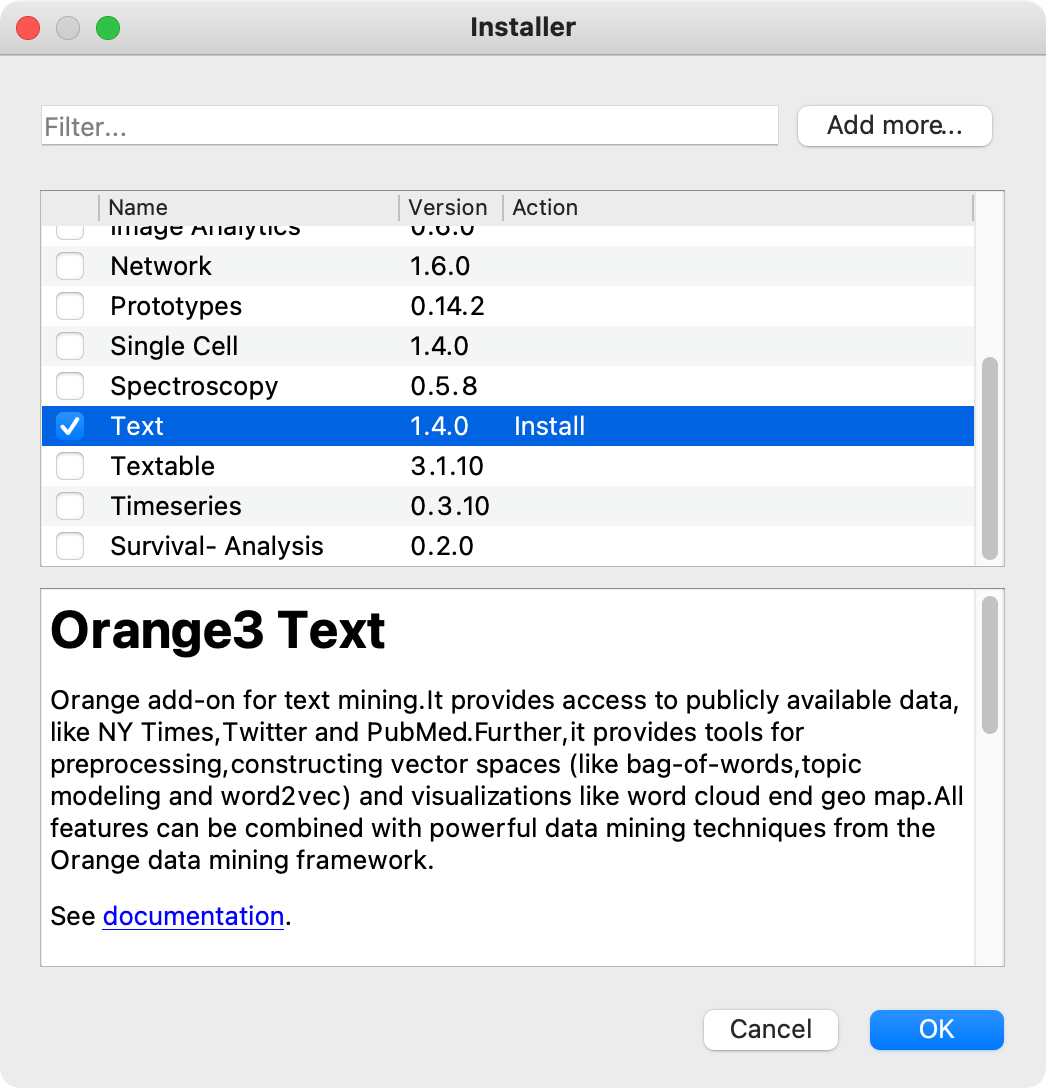
\includegraphics[width=\linewidth]{add-on-installation.png}%
  \caption{$\;$}
\end{figure}
\vspace{-0.3cm}

A new pane with widgets from the Text add-on will appear on the left side of the canvas.

\newpage

\section{Loading corpora}

A collection of text documents is called a corpus. Widget for loading corpora is called \widget{Corpus}. We will use the \emph{grimm-tales-selected} corpus, which you can select from the drop-down menu in the widget. The corpus contains 44 folk tales, collected by the Grimm brothers.

\vspace{-0.2cm}
\begin{figure}[h]
  \centering
  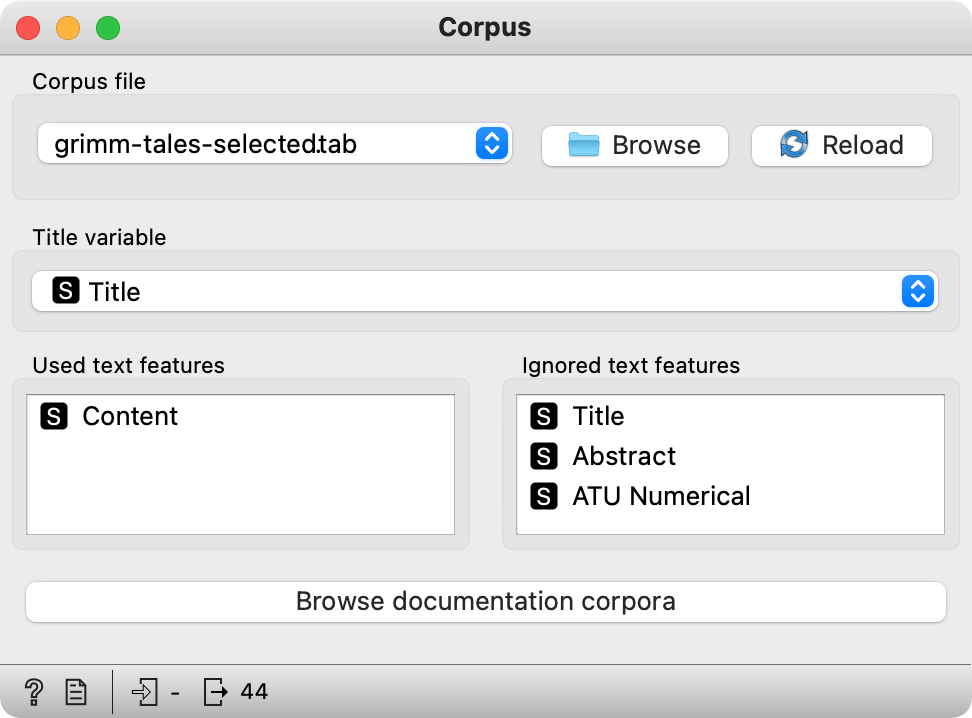
\includegraphics[width=\linewidth]{corpus.png}%
  \caption{$\;$}
\end{figure}
\vspace{-0.3cm}

The widget is very similar to the \widget{File} widget with one important distinction. Orange needs to know which attribute contains the content of the documents. The Grimm corpus has the attribute \emph{Content}, which is already placed in the \emph{Used text features} section. Alternatively, drag one or more attributes you would like to use for text mining to the box on the left.

\begin{marginfigure}
      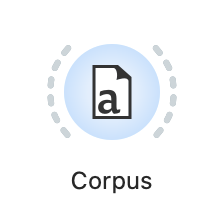
\includegraphics[width=30mm]{workflow.png}%
      \caption{$\;$}
\end{marginfigure}
